\section{Monte Carlo samples}
\label{mcgeneration}

First of all in this section we discuss the settings of the
Monte Carlo generation of the signal and background
events used in this work.
%
We also discuss how we study the effects of finite detector
resolution by means of an smearing of the final-state
particles four-momentum.

\subsection{Higgs pair production}
%%%%%%%%%%%%%%%%%%%%%%%%%%


%%%%%%%%%%%%%%%%%%%%%%%%%%%%
\begin{figure}[t]
\begin{center}
  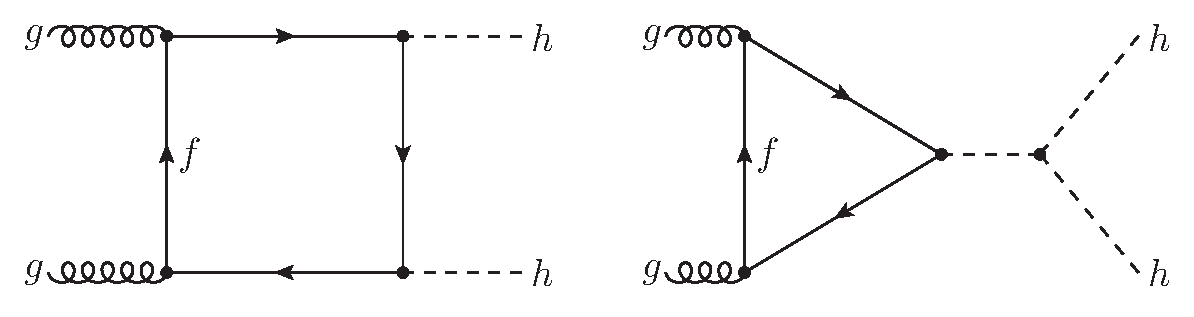
\includegraphics[width=0.90\textwidth]{plots/hhFeyn.pdf}
  \caption{\small Representative Feynman diagrams
    for Higgs pair production in gluon fusion at
    leading order.
    %
    Only the left diagram is sensitive to the trilinear coupling
    $\lambda$.
}
\label{fig:hhFeyn}
\end{center}
\end{figure}
%%%%%%%%%%%%%%%%%%%%%%%

Higgs pair production is simulated at leading order using
{\tt MadGraph5\_aMC@NLO}~\cite{Alwall:2014hca}, with finite $m_t$ effects taken into
account.\footnote{We thank Eleni Vrodynou for assistance here.}
%
This tailored {\tt MadGraph5\_aMC@NLO} model  simulates
gluon-gluon-fusion Higgs boson pair production including the effects
of the
exact form factors for the top triangle and box loops at leading
order, obtained from~\cite{Plehn:1996wb}.\footnote{Note that since recently it is possible to compute also
loop-induced processes as well without the need of special
models~\cite{Hirschi:2015iia}.}
%
We use the NNPDF 3.0 $n_f = 4$ LO set~\cite{Ball:2014uwa} with
$\alpha_S(m_Z^2)=0.118$
as interfaced via {\tt LHAPDF6}~\cite{Buckley:2014ana}.
%
We use the default settings of the renormalization and factorization
scale of the model.
%
The Higgs boson parameters are also the same in the default model,
in particular we use $m_H=125$ GeV, consistent with the latest
measurements from ATLAS and CMS~\cite{Aad:2014aba,Khachatryan:2014jba}.
%
The value of the Higgs trilinear coupling $\lambda$ is set to its
Standard Model value.
%
The calculation is performed in the
$N_f$=4 scheme and thus
takes into account the finite mass of the $b$-quarks.

The signal samples are rescaled so that the integrated cross-section matches that of the
NNLO calculation of the inclusive cross-section from Ref.~\cite{deFlorian:2013jea}:
this corresponds to using a $K$-factor $\sigma_{\rm NNLO}/\sigma_{\rm LO}=2.3$.
%
Let us note that resummed NNLO+NNLL calculations for Higgs pair production have also become available recently~\cite{deFlorian:2015moa},
leading to a moderate enhancement as compared to the fixed-order NNLO calculation.


In Fig.~\ref{fig:hhFeyn} we show representative Feynman diagrams
    for Higgs pair production in gluon fusion at
    leading order.
    %
    The non-trivial interplay between the heavy quark loop and
    the trilinear it is not immediate how to the extract
    $\lambda$ from the observation of Higgs pair
    production cross-section.


%
Parton level events are then showered with the {\tt Pythia8} Monte
Carlo~\cite{Sjostrand:2007gs,Sjostrand:2014zea}, in particular with {\tt v8.201}.
%
We use the default settings in the parton shower, in particular
we use the Monash 2013 tune~\cite{Skands:2014pea}, based on the NNPDF2.3LO PDF set~\cite{Ball:2012cx}.
%
We have switched off hadronisation, since this allows a more transparent modeling of
$b$-tagging.
%
A complete simulation of $b$-tagging at the hadron level is difficult to achieve without a full
detector simulator, which is beyond the scope of this paper.
%
For a similar reason, we don't consider underlying event, multiple parton interactions and
pile-up, which can be taken of using a variety of subtraction methods~\cite{Cacciari:2009dp}.
%
The same applies to the background samples, which we discuss now

\subsection{Backgrounds: QCD multijet and $t\bar{t}$ production}

Now we turn to discuss the Monte Carlo generation of the relevant background processes.
%
All background samples are generated at leading-order
with the {\tt SHERPA} event generator~\cite{Gleisberg:2008ta}, v2.1.1.
%
As in the case of the signal generation, the NNPDF 3.0 $n_f = 4$ LO set with strong coupling $\alpha_S(m_Z^2)=0.118$ is used for all samples.
%
Factorisation and renormalisation scales are set as $\mu_F=\mu_R=H_T/2$ for all
the samples.

We have considered all the relevant samples that can lead to the event
being tagged as a $HH\to 4b$ candidate.
%
First of all QCD we have $4b$ multi-jet production of course.
%
But also we generate QCD $2b2j$ and $4j$ multi-jet samples,
that can lead to the event being tagged in the case of multiple light
jets being mistagged as $b$-quarks.
%
While the light jet mistag probability is small, we find that
in general the $2b2j$ and $4j$ backgrounds cannot be neglected because
of their large cross-sections and enhancement from combinatorics, that
increase their contribution as compared to a naive estimate.
%
Neglecting the  $2b2j$ and $4j$ backgrounds is particularly
important for the resolved and intermediate categories, but less
so for the boosted one.
%
We don't include the NLO $K$-factor for the backgrounds but instead assume
a given experimental overall systematic uncertainties common to all backgrounds.

In addition to the QCD multijet, we also generate $t\bar{t}$ samples
in the fully hadronic final state, which lead to a $2b4j$ signature that can
contribute to the fake rates, and that has a similar topology that
the corresponding QCD sample.
%
We have used a value of the top quark mass of $m_t=173.2$ GeV.
%
Semileptonic decays of top quarks can be easily removed by requiring
a lepton veto.


At the generation level the following basic cuts are applied to
background events.
%
Each final state particle in the hard process must have $p_T \ge 20$ GeV, and be located
in the central region with
$| \eta | \le 3.0$.
%
In addition, at the matrix element level
all final state particles must be separated by a minimum $\Delta R_{\mathrm{min}} =0.1$.
%
We have checked that the generator-level cuts are loose enough as compared to the actual
analysis cuts.
%


Total cross-sections and details of the samples generated are shown in Table~\ref{tab:samples}.
%
First of all we see that the $t\bar{t}$ and QCD $4b$ samples are of
the same order of magnitude.
%
The $bbjj$ cross-section is more than a factor 200 as compared to the
$4b$ result, so in principle it should be subleading taking into
account the mistag rate, but as we will show below,
this is not true due to combinatoric.
%
 For top quark production, only the hadronic final state is generated.
  %
The $hh$ cross-section includes the NNLO $K$-factor.


%%%%%%%%%%%%%%%%%%%
\begin{table}[h]
\begin{center}
\begin{tabular}{|c|c|c|c|c|}
\hline
Process &  Generator & $N_{\mathrm{evt}}$ & $\sigma_{\mathrm{tot}}$ (pb) \\
\hline
\hline
$pp \to HH$ &  {\tt MadGraph5\_aMC@NLO} & 100K & $3.87\times10^{-2}$  \\
\hline
\hline
$pp \to b\bar{b}b\bar{b}$ &  {\tt SHERPA}v2.1.1 & 3M &$1.121 \times10^3$  \\
$pp \to b\bar{b}jj$ &  {\tt SHERPA}v2.1.1 & 3M & $2.659 \times 10^5$  \\
$pp \to jjjj$ &  {\tt SHERPA}v2.1.1 & 3M  & $9.709\times 10^6$  \\
$pp \to t\bar{t}\to b\bar{b}jjjj$ &  {\tt SHERPA}v2.1.1 & 3M & $2.514\times 10^3$ \\
\hline
\end{tabular}
\caption{\small Summary of signal and background samples generated in this work,
  together with the corresponding generator-level cross-section.
  %
  For top quark production, only the hadronic final state is generated.
  %
The $hh$ cross-section includes the NNLO $K$-factor.  
} \label{tab:samples}
\end{center}
\end{table}%
%%%%%%%%%%%%%%%%%%%%%%%%%%%%%%%%%%%%%%%%%%%

As a cross-check of the background cross-sections reported in Table~\ref{tab:samples}, we have produced leading order
multi-jet samples
using the {\tt MadGraph5\_aMC@NLO} program, and compared with the results for the same processes reported in
Ref.~\cite{Alwall:2014hca}.
%
For comparison with the latter numbers, 
we require in all samples four anti-$k_T$ $R=0.5$ jets with $p_T \ge 80 $ GeV, and the leading jet must have $p_T \ge 100$ GeV, and
also that all jets must be within an acceptance of $|\eta| \le 2.5 $.
%
We find agreement, within the scale uncertainties, between the {\tt MadGraph5\_aMC@NLO} and {\tt SHERPA} calculations of the multi-jet
backgrounds, so we can be confident that the set-up that we will use in this analysis is robust enough.



Finally, let us discuss the smearing applied to signal
and background samples.
%
It is beyond the scope of this work to perform a complete study of the impact of
detector effects in this process.
%
However, it is still important to include some form of rough estimate of detector
effects in the analysis, to properly estimate for example the impact
of the Higgs mass window cuts.
%
In this work we simulate the finite momentum resolution of the ATLAS and CMS
hadronic calorimeters by applying a Gaussian smearing to the four components
of the four-momentum $p$, with mean zero and standard deviation $\Delta p$.
%
We take as baseline value a smearing of $\Delta p=5\%$, and in
Sect.~\ref{sec:optimisation} we explore how our results change
if a more optimistic or pessimistic value is assumed for the momentum
resolution in the LHC detectors.
